\documentclass[12pt, a4paper]{article}
\usepackage[spanish,es-tabla]{babel}
\usepackage[utf8]{inputenc}
\usepackage[T1]{fontenc}
\usepackage{lmodern}
\usepackage{graphicx}

\title{Arquitectura de Microprocesadores}
\author{Gianfranco Talocchino}
\date{Marzo - Abril de 2022}

\begin{document}
\maketitle

\section{Preguntas orientadoras}
\subsection{Introducción}
\begin{enumerate}
    \item Describa brevemente los diferentes perfiles de familias de 
    microprocesadores/microcontroladores de ARM. Explique alguna de sus 
    diferencias características.
    
    La familia de arquitecturas ARM Cortex esta dividida en tres 
    principales subfamilias.
    
    \begin{itemize}
        \item Cortex A (\emph{\textbf{A}pplication}): Es la que ofrece mayor rendimiento. Está 
        orientada la ejecución de sistemas operativos como \emph{Linux} y derivados. Su 
        aplicación principal son computadoras, celulares, \emph{tablets}, etc.
        \item Cortex R (\emph{\textbf{R}eal-Time}): Esta orientada y optimizada a aplicaciones 
        \emph{real-time}. Su aplicación se centra en la industria médica, aeronáutica, etc.
        \item Cortex M (\emph{\textbf{M}icrocontrollers}): Esta orientada al uso en 
        microcontroladores y sistemas embebidos de propósito general.
    \end{itemize}
\end{enumerate}
\subsection{Cortex M}
\begin{enumerate}
    \item Describa brevemente las diferencias entre las familias de procesadores Cortex M0, M3 
    y M4.
    
    A grandes rasgos la diferencia es el costo, la velocidad y el consumo de energía. Los 
    Cortex M0 están optimizados para ocupar la menor cantidad de silicio y ser lo mas baratos 
    posible. Frente a los Cortex M3 las diferencias a nivel de Hardware se traducen en
    que algunos core peripherals son opcionales, una arquitectura de memoria Von Neumann y la 
    falta de MPU. Por otro lado, los Cortex M4 añaden la posibilidad de contar opcionalmente 
    con una FPU e instrucciones de DSP. De esta manera, entre los Cortex M0 y M4 el rendimiento
    es creciente, asi como también el costo y el consumo de energía debido a la mayor cantidad 
    de features implementadas en hardware.
    
    \item ¿Por qué se dice que el set de instrucciones Thumb permite mayor densidad de código?
    Explique
    
    El set de instrucciones Thumb permite mezclar instrucciones de 16 y 32 bits sin que exista una 
    sobrecarga asociada al cambio. Esto da lugar a que operaciones mas simples puedan ser llevadas 
    a cabo con instrucciones de 16 bits en vez de 32 bits. Como resultado, se logra 
    una mayor densidad de código que al solo utilizar instrucciones de 32 bits para operaciones 
    simples y complejas.
        
    \item ¿Qué entiende por arquitectura load-store? ¿Qué tipo de instrucciones no posee este
    tipo de arquitectura?
    
    Una arquitectura de hardware load-store es aquella que solo las instrucciones load y store 
    acceden a memoria RAM. El resto de operaciones (aritméticas, lógicas, etc ..) usan solo 
    registros internos del procesador
    
    \item ¿Cómo es el mapa de memoria de la familia?
    Los Cortex M tiene un sistema de memoria con direcciones de 32 bits que
    generan un espacio de lineal de direcciones de 4GB. El cual, está participando en 
    número de regiones asignados a diferentes usos.
    \begin{itemize}
        \item Código de programa
        \item RAM
        \item Periféricos
        \item Registros de control
    \end{itemize}
    
    \begin{figure}
        \centering
        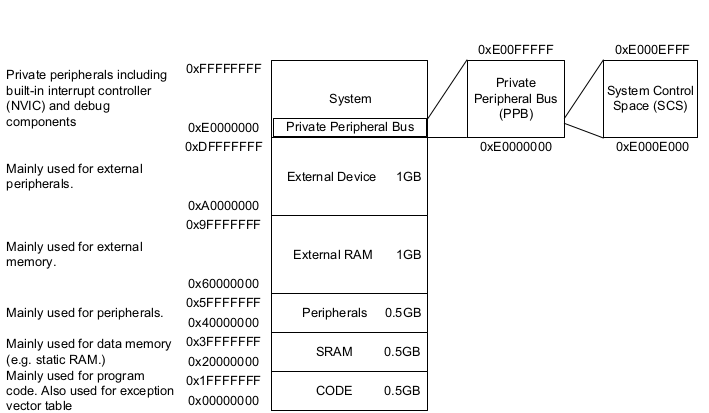
\includegraphics[scale=0.6]{map}
        \caption{Mapa de memoria de la familia Cortex M.}
        \label{fig:my_label}
    \end{figure}
    
\end{enumerate}
\end{document}

